\chapter{Soạn thảo văn bản trong \LaTeX}\label{ch:2}
\section{Cài đặt \LaTeX}\label{sec:2.1}
\subsection{Cài đặt \LaTeX\ trên Linux}\label{subsec:2.1.1}   
\renewcommand{\labelitemi}{\textbullet}
LateX có thể dễ dàng cài đặt trên Linux bằng cách cài trình soạn thảo hỗ trợ nó. Thông thường,
một số hệ điều hành nhân Linux sẽ tự động tìm kiếm và cài đặt bổ sung TeXLive nhằm khởi chạy
được trình soạn thảo đó. Ví dụ ở hình \ref{fig:kile} dưới đây sử dụng hệ điều hành Fedora.\par
\begin{figure}[H] 
 \begin{subfigure}{0.5\textwidth}
  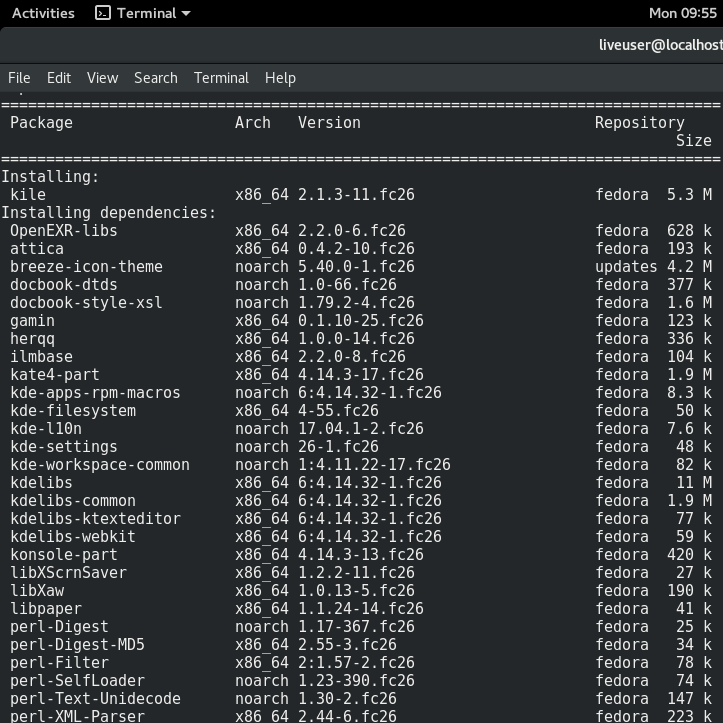
\includegraphics[width=1.\linewidth]{kile1.png}
  \caption{Kile}
  \label{fig:kile1}
 \end{subfigure}
 \begin{subfigure}{0.5\textwidth}
  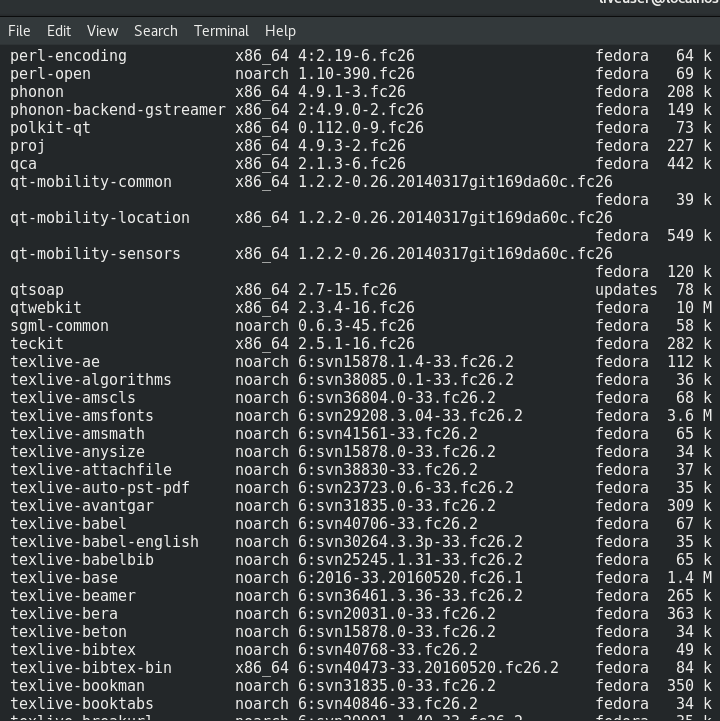
\includegraphics[width=1.\linewidth]{kile2.png}
  \caption{Các gói TeXLive}
  \label{fig:kile2}
 \end{subfigure}

 \caption{Kết quả có được sau khi nhập câu lệnh cài Kile}
 \label{fig:kile}
\end{figure}


Sau câu lệnh \verb|sudo dnf install kile|, ta có thể thấy, ngoài Kile, hệ thống tự động tìm kiếm
và tải về TeXLive và các gói chương trình khác \emph{vừa đủ} để khởi chạy trình soạn thảo trên.\par
\clearpage 
Tuy nhiên, sẽ có trường hợp ta muốn đích thân tải hay chỉ muốn tải TeXLive (bản có LaTeX) hoặc
hệ điều hành không tự động tải về. Ta có thể thực hiện như sau:\par

\begin{itemize}
 \item Đối với các hệ điều hành Debian, Ubuntu,\dots ta nhập câu lệnh sau vào terminal:
 
 \begin{verbatim}
  # apt-get install texlive texlive-base 
 \end{verbatim}
 hoặc
 \begin{verbatim}
  # apt-get install texlive-full 
 \end{verbatim}
 Câu lệnh \verb|texlive-full| sẽ tải hết tất cả các gói của LaTeX.
 \item Đối với các hệ điều hành RedHat, CentOS, Fedora,\dots ta nhập:
 \begin{verbatim}
  # yum install texlive texlive-latex 
 \end{verbatim}
 Ta có thể sẽ cần quyền admin, trường hợp đó chỉ cần thêm \verb|sudo| vào trước câu lệnh và nhập mật
 khẩu admin khi được hỏi. Đối với các bản Fedora từ 18 trở đi, nên sử dụng \verb|dnf| thay cho
 \verb|yum|.
\end{itemize}

Sau đó, nếu muốn, ta có thể tiến hành cài đặt trình soạn thảo hỗ trợ LaTeX như bình thường. Mặc định TeXLive
sau khi được cài đặt sẽ nằm ở đường dẫn \path|/usr/share/texlive|, và các gói của LaTeX sẽ nằm ở
\path|/usr/share/texlive/texmf-dist/tex/latex|.\par
Người dùng còn có thể nhập câu lệnh \verb|yum install texlive-latex-doc| (CentOS, RedHat,\dots) hoặc
\verb|apt-get install texlive-latex-doc| (Ubuntu, Debian,\dots), để tải về bộ tài liệu thông tin và
hướng dẫn cho LaTeX và các gói, lớp tiêu chuẩn. Bộ tài liệu mặc định nằm ở \path|usr/share/texlive/texmf-dist/doc/latex/base|.\par
Tương tự, để tải và cài đặt các gói LaTeX (khi được hệ thống yêu cầu để chạy tập tin \texttt{.tex}), người dùng cũng có thể sử dụng
\texttt{yum} hoặc \texttt{apt-get} kèm theo \path|install texlive-<tên gói>|, Linux sẽ tự động tìm kiếm, tải (nếu có) và cài
đặt gói mở rộng trên.

\clearpage
\subsection{Cài đặt \LaTeX\ trên Windows}\label{subsec:2.1.2}
Trên nền Windows, ta có thể chọn TeXLive làm gói phân phối LaTeX, tuy nhiên, MiKTex hỗ trợ, đồng
bộ tốt hơn cho Windows và cũng miễn phí như TeXLive, nên đối với hệ điều hành này, ta sẽ chọn
MiKTeX.\par
MiKTeX có thể được cài đặt qua các buớc sau:\par

\begin{itemize}
 \item \textsl{Bước 1}: Truy cập trang web \url{https://miktex.org/download}, để tải trình cài đặt
 (installer) cho MiKTeX. Click vào tab \textbf{All downloads} để chọn bản cài đặt phù hợp với hệ
 điều hành đang sử dụng. Nên chọn bản Net installer để có đầy đủ chức năng.
 \begin{figure}[H]
  \centering
  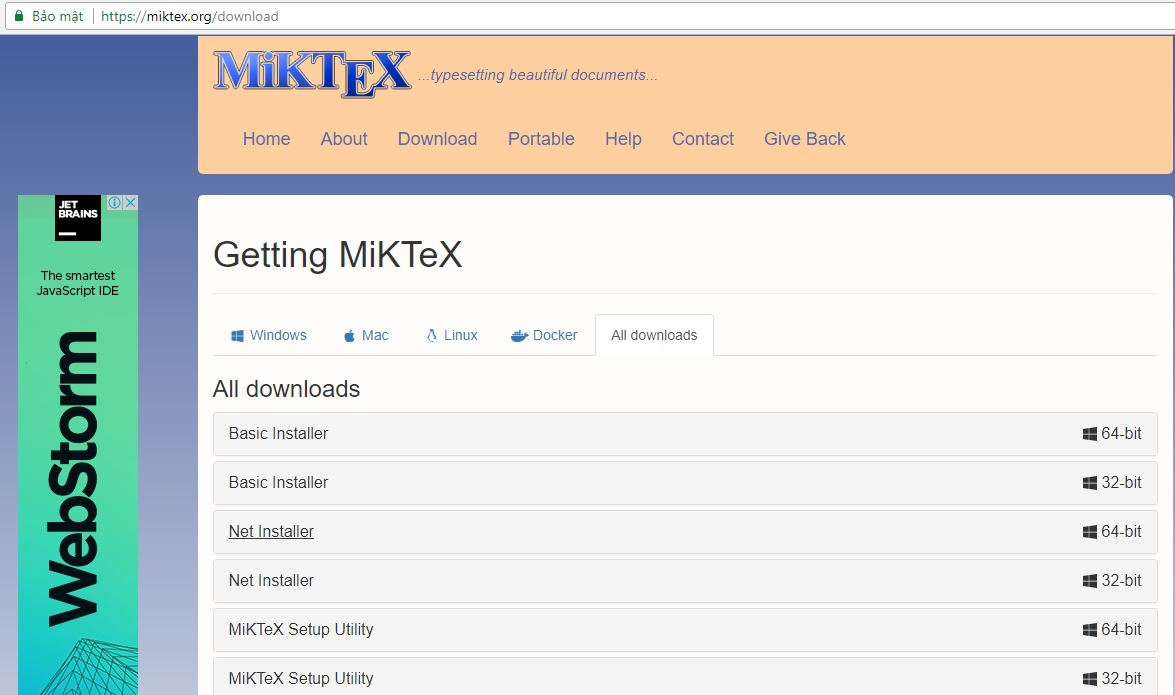
\includegraphics[width=1.\textwidth]{Capture}
  \caption{Giao diện trang tải MiKTeX}
  \label{fig:web}
 \end{figure}
 \item\hypertarget{step:2}{\textsl{Buớc 2}}: Mở installer và tiến hành cài đặt, sau khi chấp nhận điều khoản sử dụng,
 ở bước tiếp theo, có hai lựa chọn cài đặt gói có sẵn trong máy (Install MikTeX), hay tải (download) các gói từ 
 mạng (Download MiKTeX). Do đây là lần cài đặt đầu tiên, ta nên chọn tải gói về như minh hoạ ở hình \ref{fig:down}.
 \begin{figure}[H]
  \centering
  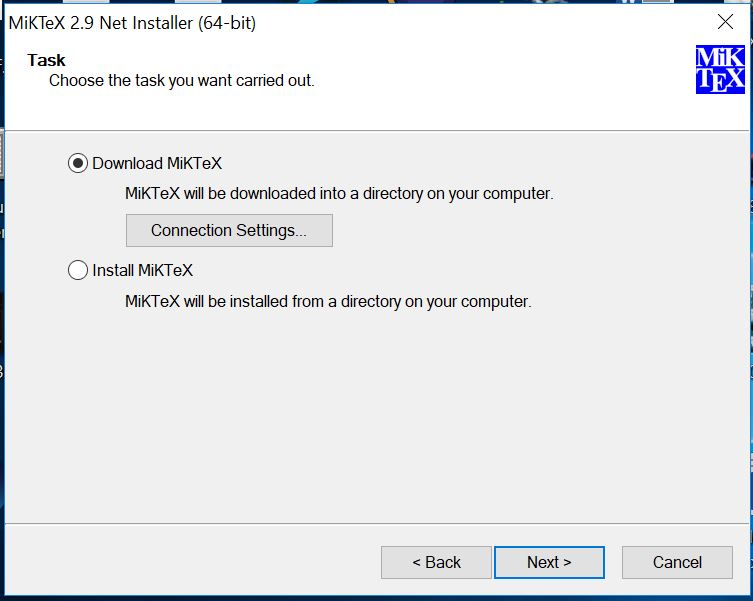
\includegraphics[width=0.68\textwidth]{install2}
  \caption{Chọn tải các gói từ mạng}
  \label{fig:down}
 \end{figure}
 \item \hypertarget{step:3}{\textsl{Buớc 3}}: Ta có hai tuỳ chọn Basic LaTeX (các gói cơ bản của LaTeX) hoặc Complete
 LaTeX (tất cả các gói chính thức của LaTeX), tuỳ theo tốc độ và nhu cầu sử dụng mà ta đưa ra
 lựa chọn, tuy nhiên, nên lựa chọn gói Basic để việc download được tiến hành nhanh chóng. MiKTeX có cơ chế tự động tải các gói còn thiếu, nếu phát hiện trong tập tin văn
 bản LaTeX sử dụng gói không có sẵn trong máy. 
 \begin{figure}[H]
  \centering
  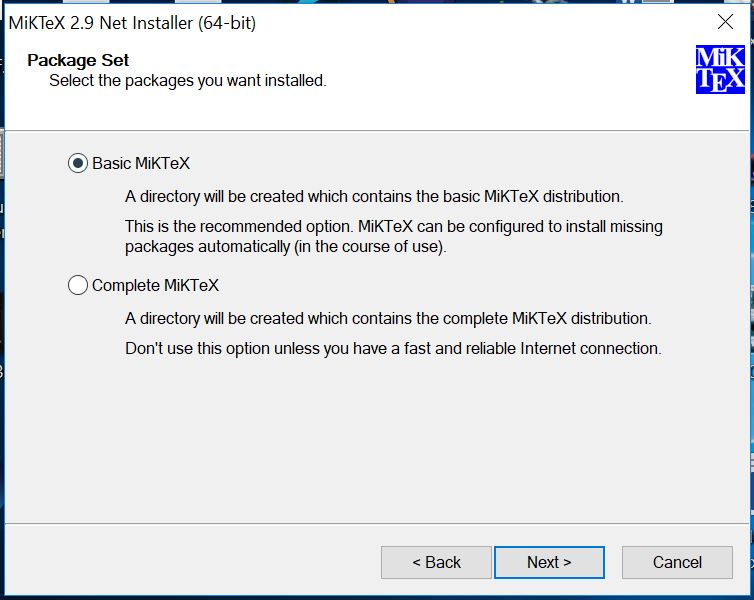
\includegraphics[width=0.68\textwidth]{install3}
  \caption{Chọn gói muốn tải}
  \label{fig:set}
 \end{figure}
 \item \textsl{Bước 4}: Sau khi chọn loại gói, tiếp theo sẽ là danh sách các nguồn cung cấp
 gói, ta nên chọn nguồn gần nhất và giao thức FTP để đảm bảo tốc độ download.
 \begin{figure}[H]
  \centering
  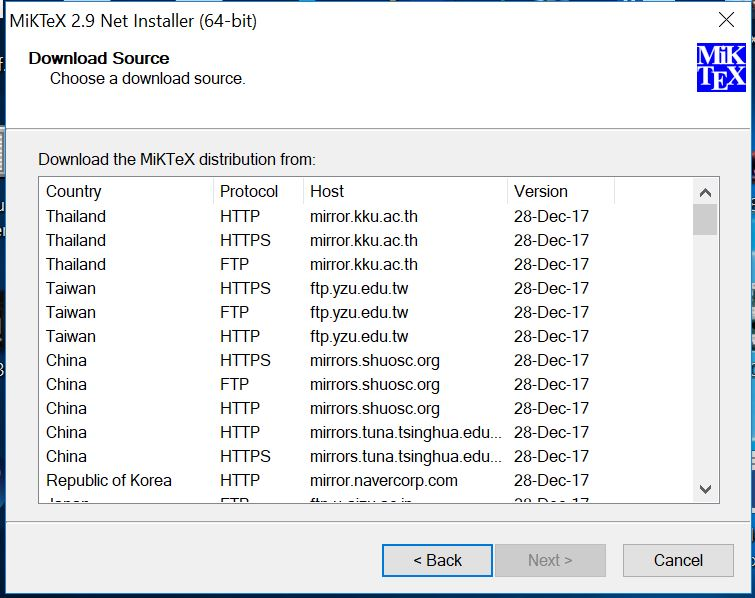
\includegraphics[width=0.68\textwidth]{install4}
  \caption{Chọn nguồn tải}
  \label{fig:source}
 \end{figure}
 \item \textsl{Bước 5}: Ở buớc này ta chỉ định đường dẫn tới thư mục mà ta muốn đặt các gói tải
 về.
 \begin{figure}[H]
  \centering
  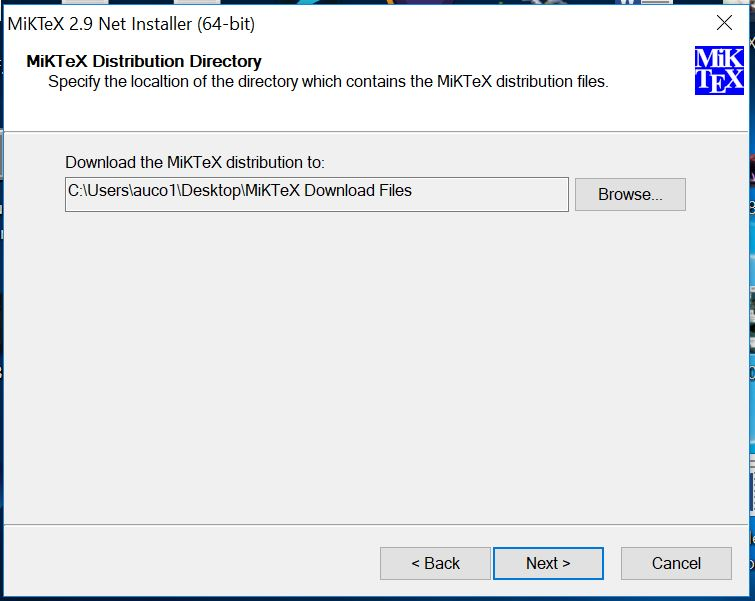
\includegraphics[width=0.68\textwidth]{install5}
  \caption{Chỉ định đường dẫn tới thư mục chứa gói đã tải về}
  \label{fig:dest}
 \end{figure}
 Sau đó, chọn \textbf{Next}, buớc kế tiếp là xác nhận thông tin, nếu không có gì cần thay đổi, ta
 bấm \textbf{Start} để tiến hành tải gói.
 \begin{figure}[H]
  \centering
  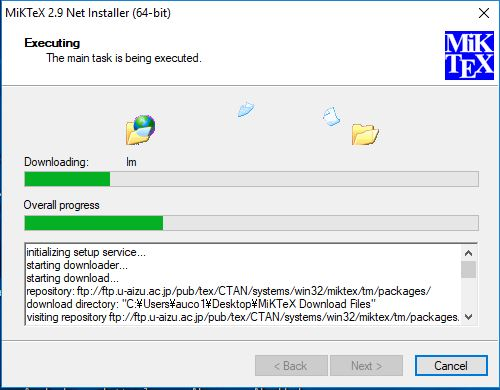
\includegraphics[width=0.68\textwidth]{install7}
  \caption{Quá trình download đang được tiến hành}
  \label{fig:downloading}
 \end{figure}
 \item \textsl{Bước 6}: Lặp lại bước \hyperlink{step:2}{2}, nhưng lần này chọn tuỳ chọn \textbf{Install MiKTeX}.
 \begin{figure}[H]
  \centering
  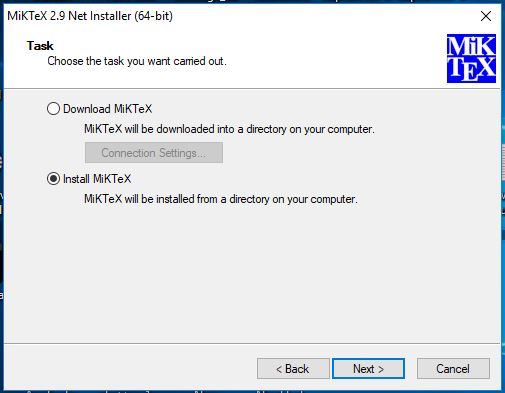
\includegraphics[width=0.68\textwidth]{install8}
  \caption{Chọn tuỳ chọn cài đặt MiKTeX}
  \label{fig:install}
 \end{figure}
 \clearpage 
 \item \textsl{Bước 7}: Chọn gói cài đặt ứng với gói mà ta đã tải về ở buớc \hyperlink{step:3}{3}.
  \begin{figure}[H]
  \centering
  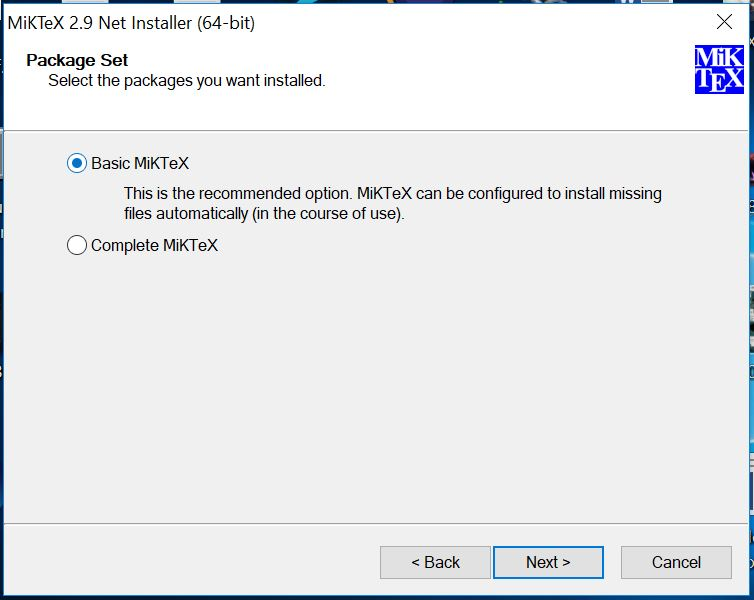
\includegraphics[width=0.68\textwidth]{install9}
  \caption{Chọn gói MiKTeX cần cài đặt}
  \label{fig:installset}
  \end{figure}
  Sau đó, chọn quyền truy cập MiKTeX cho phép ai cũng sử dụng được (Anyone\dots) hoặc chỉ tài khoản hiện tại
  (Only for:\dots).
  \begin{figure}[H]
  \centering
  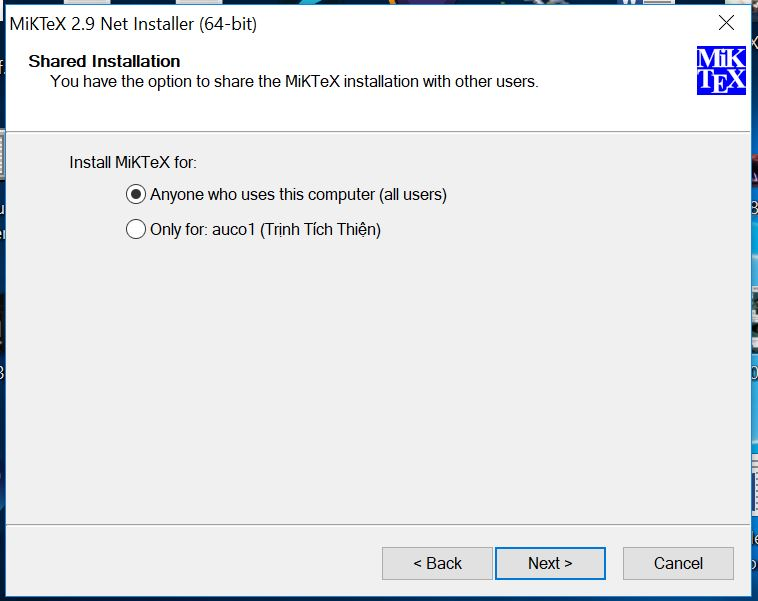
\includegraphics[width=0.68\textwidth]{install10}
  \caption{Chọn quyền truy cập MiKTeX}
  \label{fig:share}
  \end{figure}
  \clearpage 
  \item \textsl{Bước 8}: Tiếp theo, trỏ đường dẫn tới thư mục mà ta đã tải các gói về.
  \begin{figure}[H]
  \centering
  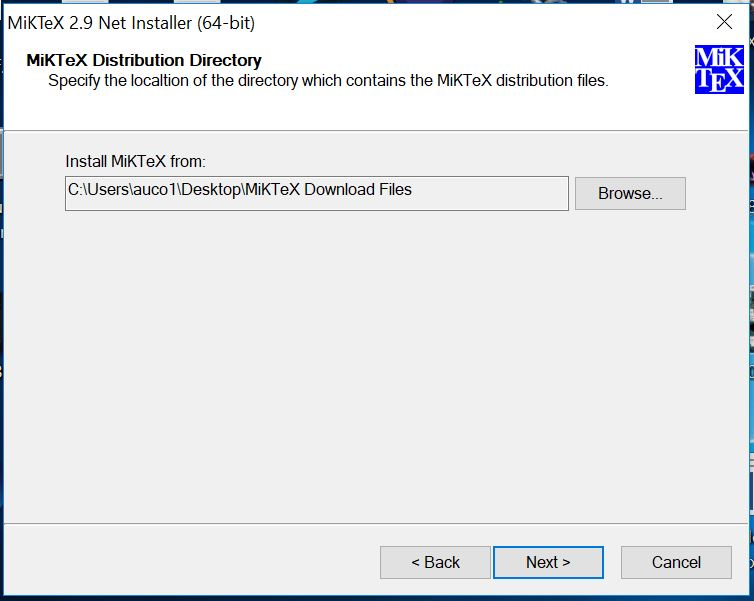
\includegraphics[width=0.68\textwidth]{install11}
  \caption{Trỏ đường dẫn tới thư mục chứa các gói}
  \label{fig:packdest}
  \end{figure}
  Sau đó, chọn đường dẫn tới thư mục ta muốn cài đặt MiKTeX.
  \begin{figure}[H]
  \centering
  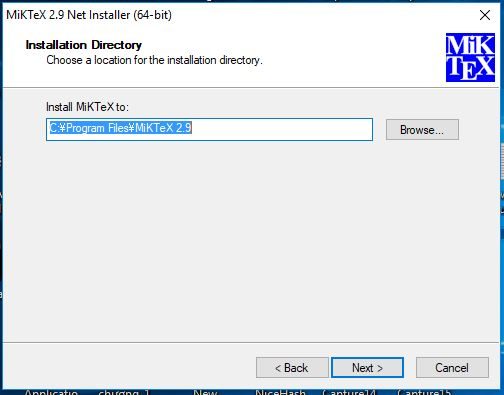
\includegraphics[width=0.68\textwidth]{install12}
  \caption{Chọn thư mục cài đặt}
  \label{fig:insdest}
  \end{figure}
  \clearpage 
  \item \textsl{Bước 9}: Ở bước này ta chọn khổ giấy mặc định (ở đây chọn A4) và các tuỳ chọn cho
  phép (Yes) hay không cho phép (No) hệ thống tự động tải g còn thiếu hoặc hỏi ý kiến trước
  khi tải (Ask me first).
  \begin{figure}[H]
  \centering
  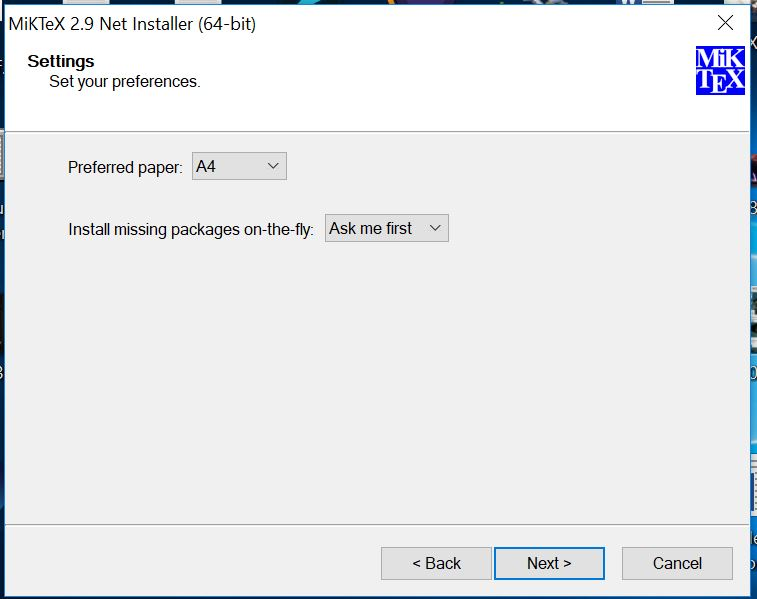
\includegraphics[width=0.68\textwidth]{install13}
  \caption{Chọn khổ giấy mặc định và tự động tải}
  \label{fig:prefer}
  \end{figure}
  \item \textsl{Bước 10}: Tới bước xác định thông tin, ta bấm \textbf{Start} để tiến hành cài đặt
  nếu không cần phải thay đổi gì.
  \begin{figure}[H]
  \centering
  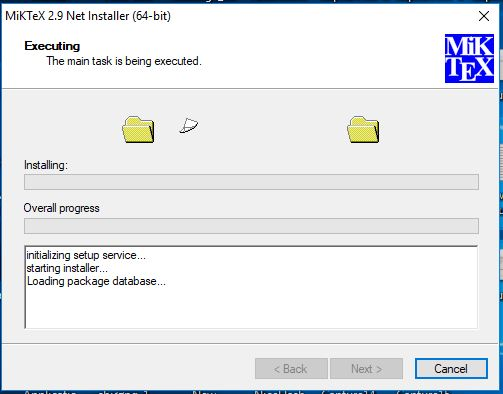
\includegraphics[width=0.68\textwidth]{install15}
  \caption{Quá trình cài đặt đang được tiến hành}
  \label{fig:installing}
  \end{figure}
  Sau khi cài đặt hoàn tất, thông báo cài đặt sẽ hiện lên, ta chọn \textbf{Close} để kết thúc quá trình
  cài đặt.
\end{itemize}

Khi đã hoàn tất cài đặt MiKTeX, ta cần chọn trình soạn thảo LaTeX hỗ trợ Windows, ngoài các trình
bản quyền, ta cũng có các trình mã nguồn mở, miễn phí. Trong các trình soạn thảo LaTeX mã nguồn mở cho Windows,
TeXstudio được sử dụng thường xuyên nhất, người dùng quan tâm có thể tham khảo và tải trình soạn thảo này tại
\url{https://www.texstudio.org/}.\par 

\section{Hướng dẫn sơ lược}\label{sec:2.2}
\subsection{Đặc điểm của \LaTeX}\label{subsec:2.2.1}
Khác với các trình soạn thảo hay xử lý văn bản ngày nay, cho phép ta được nhìn thấy hình thức trình
bày của văn bản trong quá trình soạn thảo (hay còn được gọi là “\acrshort{wysiwyg}”), với LaTeX, ta 
để việc thiết kế, định dạng cho các macro bằng việc sử dụng các câu lệnh để đánh dấu (hay mô tả, định danh) 
ý nghĩa, mục đích của nội dung mà ta soạn thảo, cũng giống như HTML.\par 
Sử dụng các câu lệnh của LaTeX, ta viết ra một tập tin chứa nội dung và các “mô tả” đó bằng các trình soạn thảo 
hỗ trợ, các tập tin đó có tên mở rộng (extension) là \verb|.tex| hay còn được gọi là tập tin đầu vào LateX 
(input file). Các tập tin đầu vào sau đó sẽ được biên dịch ra mã TeX bởi các trình soạn thảo, sử dụng các macro và 
định nghĩa có trong gói phân phối và xây dựng/chạy (build) thành tập tin văn bản (dvi, pdf,\dots) 
dùng để đọc và in. Ta lấy ví dụ một đoạn văn bản sau:\par 
\begin{verbatim}
 Tiêu đề của văn bản này
 Nguyễn Văn A
 Tháng 9 2015
 
 Hello World!
\end{verbatim}

Với các trình xử lý văn bản \acrshort{wysiwyg}, trước tiên ta sẽ chọn font, cỡ chữ,\dots cũng như
các hiệu ứng khác nhau nhằm gợi ý người đọc ý nghĩa của nội dung (ví dụ tên người thì in nghiêng,
tiêu đề cỡ chữ to, in đậm, căng lề giữa,\dots). Đối với LaTeX, ta sẽ trình bày trong tập tin đầu vào như sau:\par
\clearpage
\begin{verbatim}
\documentclass{article}
\usepackage[utf8]{inputenc}
\usepackage[vietnamese]{babel}
\title{Tiêu đề của văn bản này}
\author{Nguyễn Văn A}
\date{Tháng 9 2015}
\begin{document}
   \maketitle
   Hello World!
\end{document}
\end{verbatim}

Bằng việc khai báo như trên, ta như ngụ ý với LaTeX rằng:\par
\begin{itemize}
 \item Văn bản này là một bài báo (article).
 \item Sử dụng gói \verb=inputenc= với tuỳ chọn (option) \textbf{utf8} để xử lý các kí tự UTF-8\footnote{UTF-8 là phương thức mã hoá phổ biến để miêu tả bảng mã Unicode trong bộ nhớ}.
 \item Sử dụng gói \verb=babel= với tuỳ chọn \verb=vietnamese= hỗ trợ định dạng tiếng Việt.
 \item Tiêu đề của nó là “Tiêu đề của văn bản này”.
 \item Người viết là “Nguyễn Văn A”.
 \item Văn bản được viết vào tháng 9, 2015.
 \item Nội dung văn bản bao gồm tiêu đề và Hello World!
\end{itemize}

Dựa vào những mô tả trên, hệ thống biên dịch sẽ tìm kiếm định nghĩa của các câu lệnh trên trong
tập tin của lớp (class) \texttt{article} (tức lớp LaTeX dùng để viết bài báo), lớp là một gói tập tin đặc biệt của LaTeX, định nghĩa các câu lệnh cơ bản
và cần thiết cho một văn bản. Ngoài ra, hệ thống còn tìm kiếm trong gói \verb=babel= và \verb=inputenc=
cách định dạng và mã hoá tiếng Việt. Sau khi chạy (build) tập tin \verb=.tex= trên ta được văn bản như hình
\ref{fig:hello}.\par

\begin{figure}[ht]
 \centering
 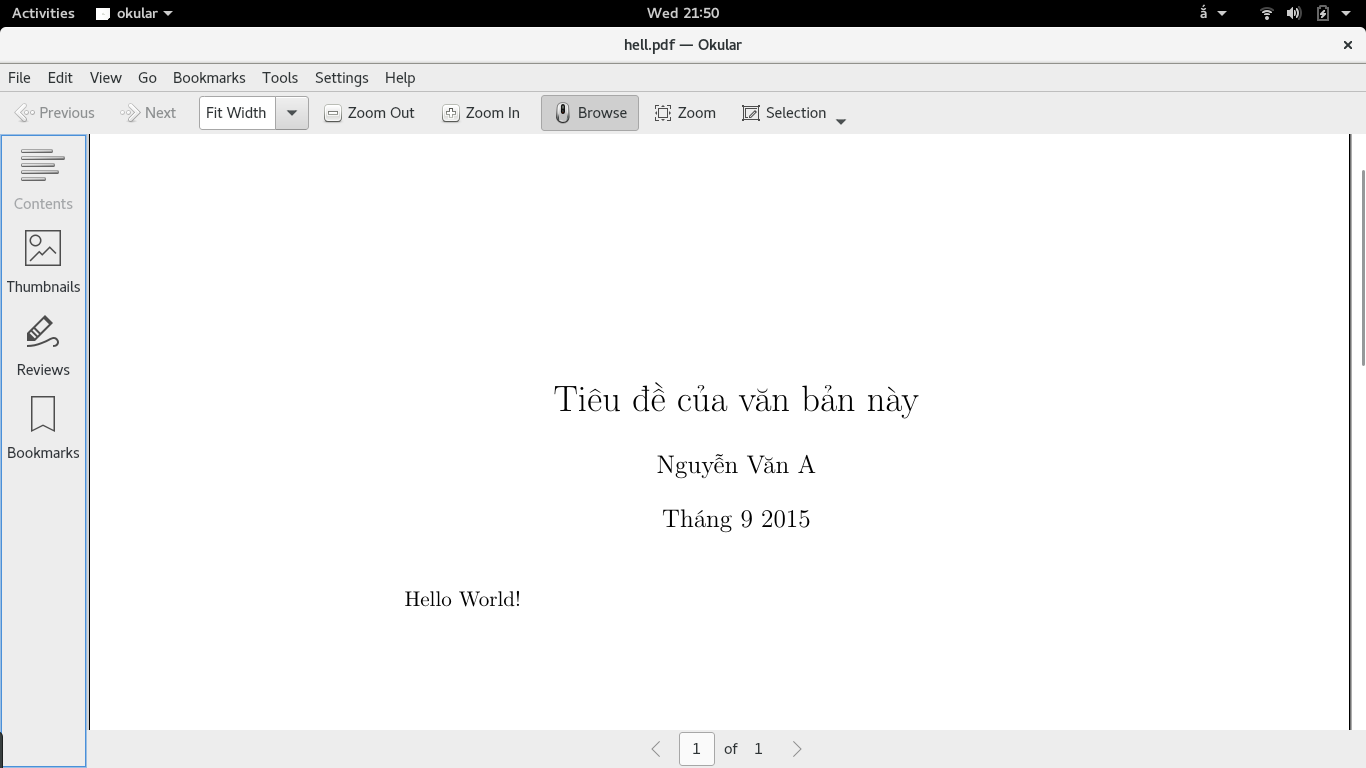
\includegraphics[width=0.9\textwidth]{hello}
 \caption{Kết quả sau khi chạy tập tin đầu vào}
 \label{fig:hello}
\end{figure}

LaTeX tự động đưa ra những định dạng khác nhau cho từng đối tượng của văn bản mà không cần ta đích
thân làm công việc đó. Tất cả những gì cần làm là nhập nội dung và “nói” cho LaTeX biết nội dung
đó thật ra là gì. Là tiêu đề, hay nội dung bình thường của bài báo.\par
Như đã đề cập ở \hyperlink{logic}{1.3}, LaTeX và TeX đã giới thiệu khái niệm logical design, tức người dùng
chỉ nên tập trung vào cấu trúc logic và nội dung văn bản hơn là định dạng, trái với visual design
(hay còn được gọi là thiết kế hình ảnh) thường thấy ở các trình soạn thảo \acrshort{wysiwyg}. Đối với các văn bản 
ngắn, cần đòi hỏi nhiều hiệu ứng, các trình soạn thảo \acrshort{wysiwyg} là thích hợp, nhưng khi
đối diện với các văn báo cáo khoa học, với nhiều kí hiệu và phương trình phức tạp, các trình soạn
thảo thông thường sẽ khiến người dùng tốn nhiều công sức trong việc tìm kiếm, bổ sung, định dạng
các kí hiệu và phương trình đó.\par 
Bên cạnh các kí hiệu khoa học, LaTeX còn hỗ trợ các câu lệnh và gói\footnote{Một số gói không có sẵn trong gói phân phối và phải được tải bổ sung} cho phép người dùng tạo 
siêu liên kết (hyperlink) đến nội bộ văn bản hoặc bên ngoài, tự động tổng hợp và tạo danh mục hình ảnh, bảng, mục lục
chỉ với một câu lệnh duy nhất, tạo, trình bày, kiểm soát danh sách tài liệu tham khảo (reference hay
bibliography), và giúp bố cục trình bày được đồng nhất xuyên suốt văn bản.\par 
Ta xét một ví dụ sau:
\begin{equation*}
 \mathcal{L}_{quarks} = \left[i\bar{\psi}_{r}\gamma^{\mu}\partial_{\mu}\psi_{r} - m\bar{\psi}_{r}\psi_{r}\right] + \left[i\bar{\psi}_{b}\gamma^{\mu}\partial_{\mu}\psi_{b} - m\bar{\psi}_{b}\psi_{b}\right] + \left[i\bar{\psi}_{g}\gamma^{\mu}\partial_{\mu}\psi_{g} - m\bar{\psi}_{g}\psi_{g}\right]
\end{equation*}

Đối với các trình soạn thảo thông thường, ta sẽ phải tốn nhiều thời gian chỉ để tìm kiếm các kí tự,
canh chỉnh các dấu gạch (---) sao cho phù hợp, hoặc để nhanh gọn, có thể chụp phương trình trên ở đâu
đó và bổ sung vào văn bản như một ảnh kèm vào nội dung nhưng khi đó ta cũng không thể chỉnh sửa được.
Để hiển thị phương trình trên bằng LaTeX, ta chỉ cần nhập:\par
\begin{lstlisting}[numbers=none]
 \mathcal{L}_{quarks} = \left[i\bar{\psi}_{r}\gamma^{\mu}\partial_{\mu}\psi_{r} - m\bar{\psi}_{r}\psi_{r}\right] + \left[i\bar{\psi}_{b}\gamma^{\mu}\partial_{\mu}\psi_{b} - m\bar{\psi}_{b}\psi_{b}\right] + \left[i\bar{\psi}_{g}\gamma^{\mu}\partial_{\mu}\psi_{g} - m\bar{\psi}_{g}\psi_{g}\right]
\end{lstlisting}

Đúng là khi nhìn vào lệnh LaTeX sẽ thấy phức tạp hơn, nhưng rõ ràng việc này giúp ta dễ dàng chỉnh sửa
nếu có sai sót cũng như không cần phải bỏ công định dạng. Khi ta biết rõ được chức năng của từng câu lệnh trên, việc
đánh ra những công thức phức tạp như vậy sẽ đơn giản và tiết kiệm thời gian hơn nhiều so với sử dụng
các trình soạn thảo truyền thống.\par
Tuy nhiên, không thể phủ định khuyết điểm của LaTeX đó là: ta chỉ có thể biết được văn bản trông như
thế nào sau khi hoàn tất quá trình biên dịch tập tin đầu vào. Người dùng có xu huớng muốn nhìn thấy kết
quả tức thì khi họ soạn thảo để dễ dàng kiểm soát cả nội dung lẫn định dạng. Các trình soạn thảo 
LaTeX và máy tính ngày nay đã phần nào giải quyết được vấn đề trên, vì việc biên dịch và xử lý
tập tin LaTeX giờ đã diễn ra gần như tức thì, chỉ với một nút bấm hay phím tắt, người soạn thảo có
thể thấy được ngay văn bản đã định dạng của mình. Các trình soạn thảo nền web thậm chí còn cung cấp giao
diện soạn thảo song song, giúp ta thấy văn bản kết quả cùng lúc với câu lệnh đánh ra.\par
\subsection{Soạn thảo văn bản}\label{subsec:2.2.2}
Phần hướng dẫn dưới đây được tham khảo từ \cite{sharelatex}. Người dùng có thể vào trang hướng dẫn
của ShareLaTeX\footnote{\url{https://www.sharelatex.com/learn}}, các diễn đàn như TeX Stack Exchange\footnote{\url{https://tex.stackexchange.com/}} 
hoặc tài liệu \cite{lamport} và \cite{latex-comp} để tham khảo thêm nhiều tính năng và câu lệnh cũng như đặt câu hỏi về TeX và LaTeX.\par
\subsubsection*{Cấu trúc cơ bản của một tập tin \LaTeX}
Điều đầu tiên ta cần làm là tạo một tập tin \verb=.tex=, sử dụng bất kì trình soạn thảo nào (ưu tiên sử dụng các trình soạn thảo
LaTeX vì chúng sẽ hỗ trợ gợi ý, tự động điền câu lệnh, highlight từ khoá và có các công cụ biên dịch).
Ta xét ví dụ cơ bản sau:\par
\begin{verbatim}
\documentclass{article}
 
\begin{document}
First document. This is a simple example, with no 
extra parameters or packages included.
\end{document}
\end{verbatim}
Và được kết quả như hình \ref{fig:vidu}.\par
\begin{figure}[H]
 \centering
 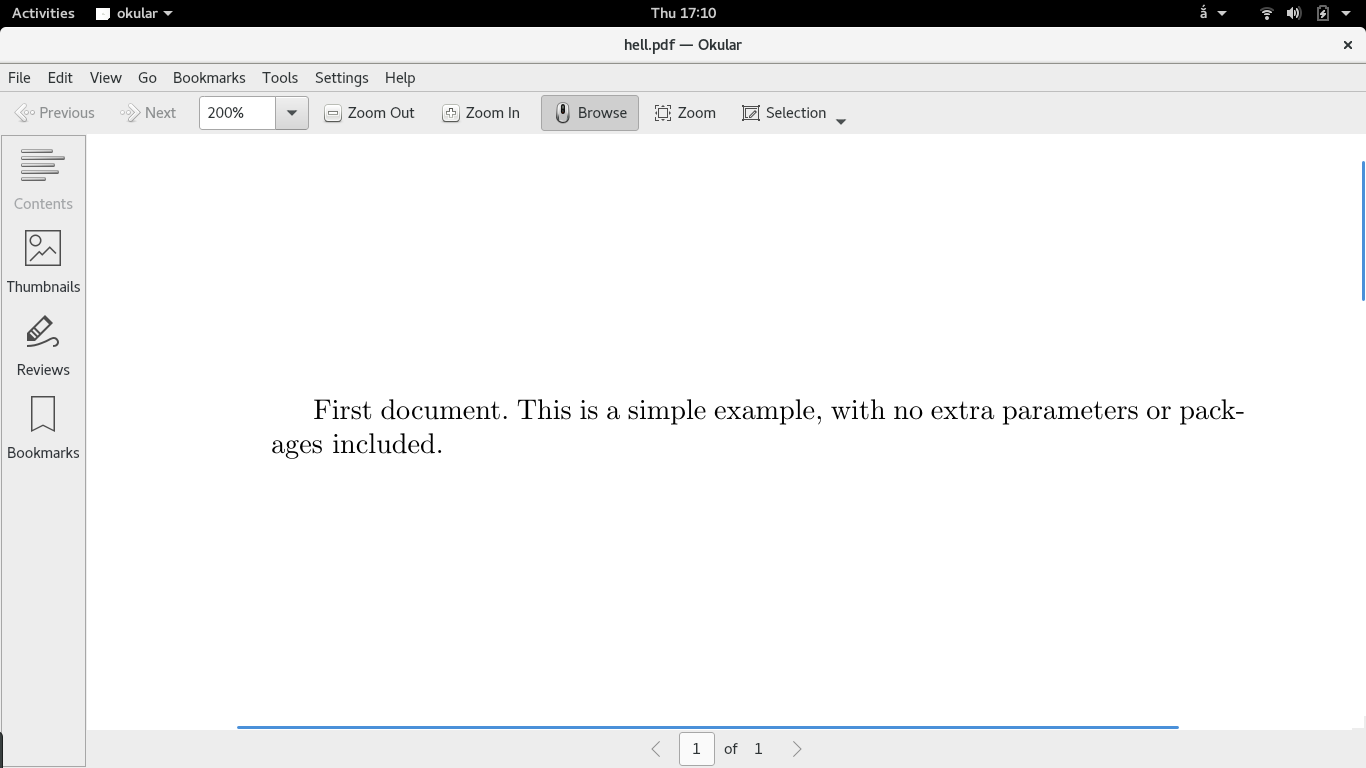
\includegraphics[width=0.9\textwidth]{vidu}
 \caption{Ví dụ một văn bản LaTeX đơn giản}
 \label{fig:vidu}
\end{figure}

Ta có thể thấy LaTeX tự động canh lề và thụt đầu dòng cho đoạn văn. Khi viết tập tin đầu vào, điều đầu
tiên ta cần làm là khai báo lớp của văn bản với câu lệnh \verb=\documentclass[option]{class}=, trong
đó, \textsl{option} đóng vai trò như thông số (hoặc \textsl{tuỳ chọn, tính năng}) của lớp có thể được bỏ trống, mỗi lớp
sẽ có các \textsl{option} khác nhau, và \textsl{class} là tên của lớp mà ta muốn sử dụng.
Thông thường, tên lớp sẽ ứng với loại văn bản mà người dùng muốn soạn thảo như \verb=article= (bài báo) hoặc
\verb=book= (sách), \verb=report= (báo cáo),\dots Mỗi lớp sẽ có thêm các câu lệnh hoặc môi trường riêng (ngoài các câu lệnh chung cơ bản) 
quyết định định dạng và bố cục tổng thể của văn bản.\par
Tiếp đến là nội dung, nội dung bình thường của văn bản sẽ được viết giữa hai câu lệnh \verb=\begin{document}= và
\verb=\end{document}=, bất kì câu lệnh hay nội dung nào được đánh vào giữa hai câu lệnh này đều được xem là “thân” 
(body) của văn bản và sẽ được hiển thị trong kết quả.\par
Tiếp theo, ta quay lại ví dụ đầu tiên ở \ref{subsec:2.2.1} với một số thay đổi:
\begin{verbatim}
\documentclass[12pt, a4paper]{article}
\usepackage[utf8]{inputenc}
\usepackage[vietnamese]{babel}
\title{Tiêu đề của văn bản này}
\author{Nguyễn Văn A}
\date{Tháng 9 2015}
\begin{document}
   \maketitle
   Hello World!
\end{document}
\end{verbatim}

Trong một tập tin LaTeX, phần trước câu lệnh \verb=\begin{document}= được gọi là \textsl{tiền tố} (\textsl{preamble}).
Ở phần tiền tố này, ta tiến hành các khai báo lớp, gói và sử dụng các câu lệnh với mục đích cung cấp thông số dưới dạng \textsl{từ khoá-giá trị}
(\textsl{key-value}) hoặc nội dung (nếu có) cho gói và lớp.\par
\begin{verbatim}
\documentclass[12pt, a4paper]{article}
\end{verbatim}

Ở đây lớp \texttt{article} đã được khai báo thêm hai tuỳ chọn, đó là \textbf{a4paper} và \textbf{12pt}. Các 
tuỳ chọn này phải được cách nhau bởi dấu phẩy (,). Trong ví dụ này, \textbf{12pt} là cỡ chữ, 
còn \textbf{a4paper} là khổ giấy sẽ được in ra trong văn bản đầu ra (output), ở đây là khổ giấy A4. Lớp \verb=article=
hỗ trợ các cỡ chữ \textbf{9pt, 10pt, 11pt} và \textbf{12 pt}, nếu để trống, mặc định sẽ là \textbf{10pt}. Ngoài khổ giấy A4, 
\verb=article= còn hỗ trợ nhiều khổ giấy khác như \textbf{letterpage}, mọi chi tiết về các tuỳ chọn
và thông tin của lớp này và tất cả các lớp cơ bản của LaTeX đều nằm trong tài liệu hường dẫn \cite{class}.\par
\begin{verbatim}
\usepackage[utf8]{inputenc}
\usepackage[vietnamese]{babel}
\end{verbatim}

Hai câu lệnh \verb=\usepackage[option]{package}= cũng tương tự như \verb=\documentclass= với hai đầu
vào \textsl{option}, là các tuỳ chọn thêm không bắt buộc, và \textsl{package} là tên gói ta muốn sử dụng.
Không như \verb=\documentclass= vốn là câu lệnh bắt buộc (và phải luôn được khai báo đầu tiên), ta không nhất thiết
phải khai báo gói, tuy nhiên, khai báo gói vẫn rất cần thiết vì sẽ có trường hợp (nếu không muốn nói là thường xuyên) ta cần
các gói bên ngoài bổ sung thêm nhiều chức năng cho LaTeX để hoàn thành các văn bản phức tạp.\par Ví dụ trên sử
dụng gói \verb=inputenc=, đây là gói chứa các bộ mã hoá (encoding) các kí tự văn bản, tuỳ chọn \textbf{utf8} 
báo cho gói biết dùng chuẩn mã hoá UTF-8, ta thường không lường trước được trong văn bản sẽ xuất hiện
kí tự đặc biệt gì hay không, cho nên gói này thường xuyên được sử dụng trong các văn bản. Gói tiếp theo
là gói hỗ trợ đa ngôn ngữ \verb=babel=. Khi văn bản có xuất hiện ngôn ngữ không phải tiếng anh, \verb=babel=
sẽ kết hợp với \verb=inputenc= để xử lý ngôn ngữ đó, tuỳ chọn của gói \texttt{babel} phần nhiều là tên của các ngôn ngữ được 
định nghĩa trong tập tin của gói (như \textbf{vietnamese} hay \textbf{english}).\par
Mọi chi tiết của hai gói trên người dùng có thể tham khảo trong tài liệu hướng dẫn của từng gói \verb=inputenc= \cite{inputenc},
\verb=babel= \cite{babel}.\par
\begin{verbatim}
\title{Tiêu đề của văn bản này}
\author{Nguyễn Văn A}
\date{Tháng 9 2015}
\end{verbatim}

Ba câu lệnh này cung cấp nội dung cho lớp \verb+article+ định dạng, chính vì thế chúng chỉ nên được đặt
ở tiền tố, dựa trên định nghĩa của từng câu lệnh này, trong tập tin định nghĩa của lớp, mà LaTeX sẽ tiến hành định dạng mẫu nội dung
được “đánh dấu”. Đúng như tên gọi, \verb=\title{text}= dùng để cung cấp cho lớp tiêu đề văn bản, \verb=\author{text}=
là tác giả và \verb=\date{text}= là thời gian văn bản được viết. Ba khai báo trên sẽ không xuất hiện trong văn bản
đầu ra cho tới khi người dùng nhập lệnh \verb=\maketitle= trong \verb=\begin{document}=. Khi bắt gặp
câu lệnh \verb=\maketitle=, LaTeX sẽ định dạng các thông tin được cung cấp ở tiền tố và in ra kết quả.\par

\subsubsection*{Các định dạng cơ bản}
Ta sẽ điểm qua ba câu lệnh định dạng cơ bản trong LaTeX:\par
\begin{itemize}
 \item \textbf{In đậm} (\textbf{Bold}): Nhập đoạn cần in đậm vào câu lệnh \verb=\textbf{text}= (viết
 tắt của text bold font).
 \item \textit{In nghiêng} (\textit{Italics}): Ta sử dụng câu lệnh \verb=\textit{text}= để đánh dấu đoạn văn
 bản cần in nghiêng.
 \item \underline{Gạch dưới} (\underline{Underline}): Câu lệnh \verb=\underline{text}= giúp đánh dấu đoạn
 văn bản cần gạch dưới.
\end{itemize}

Ví dụ một đoạn sử dụng các lệnh trên như sau:\par
\begin{verbatim}
\begin{document}
Some of the \textbf{greatest}
discoveries in \underline{science} 
were made by \textbf{\textit{accident}}.
\end{document}
\end{verbatim}

Kết quả cho ra như hình \ref{fig:basicformat}:\par
\begin{figure}[H]
 \centering
 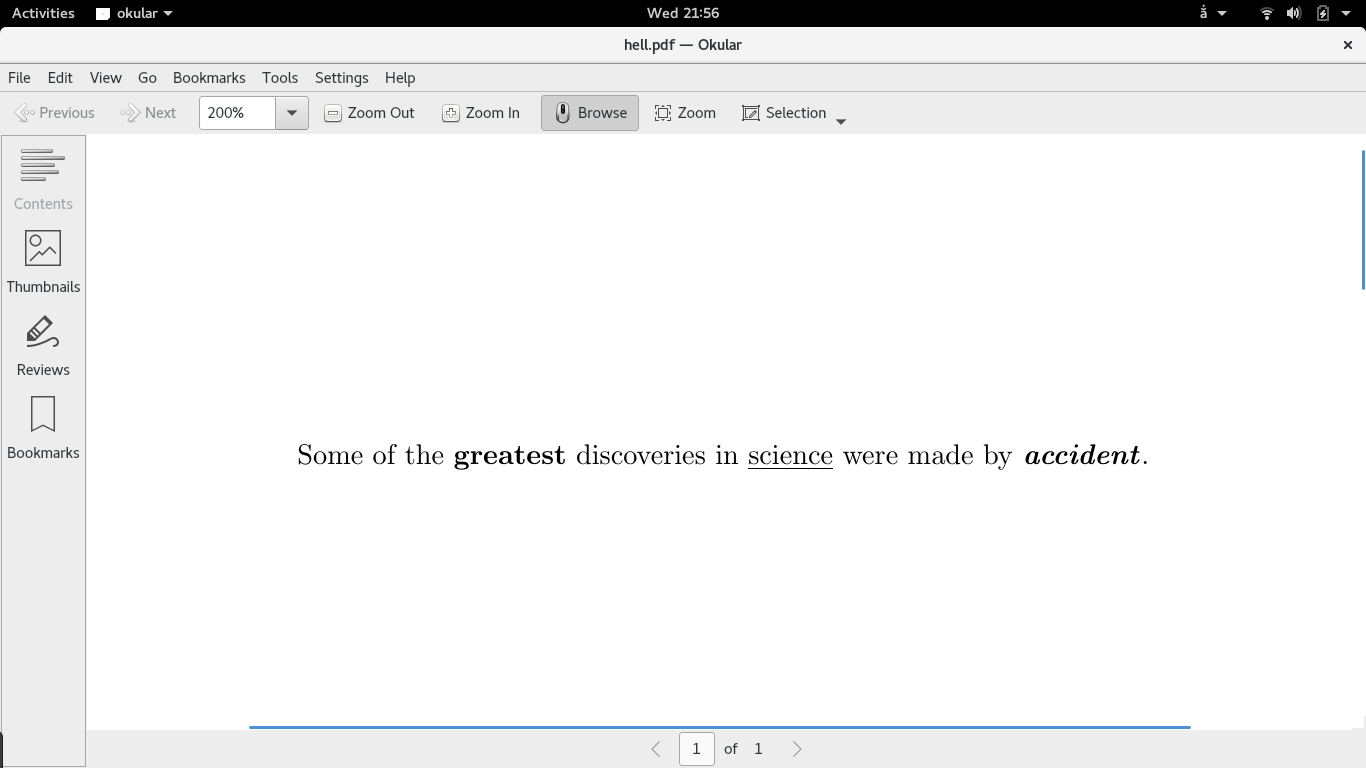
\includegraphics[width=0.9\textwidth]{basicformat}
 \caption{Văn bản đầu ra được định dạng bằng các lệnh cơ bản}
 \label{fig:basicformat} 
\end{figure}

Ngoài ba câu lệnh trên, ta còn có \verb=\emph{text}=, câu lệnh này sẽ định dạng đầu vào của nó phụ thuộc
vào tình trạng định dạng của đoạn văn chứa nó, với đoạn văn có định dạng bình thường, \verb=\emph= sẽ định
dạng in nghiêng, dưới đây là ví dụ sử dụng câu lệnh ở các trường hợp khác nhau:\par
\clearpage 
\begin{verbatim}
\begin{document}
Some of the greatest \emph{discoveries} 
in science 
were made by accident.
 
\textit{Some of the greatest \emph{discoveries} 
in science 
were made by accident.}
 
\textbf{Some of the greatest \emph{discoveries} 
in science 
were made by accident.}
\end{document}
\end{verbatim}
\begin{figure}[H]
 \centering
 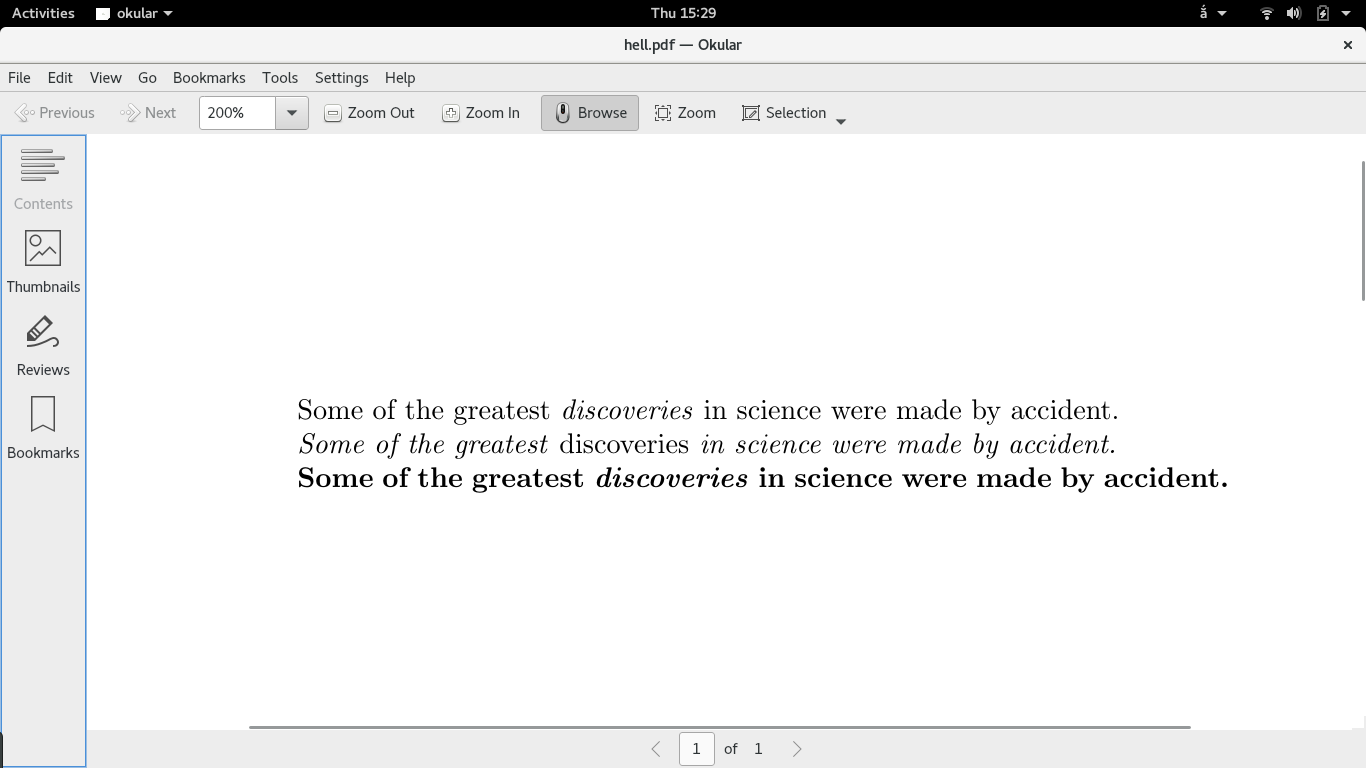
\includegraphics[width=0.9\textwidth]{emph}
 \caption{Ví dụ cho câu lệnh \texttt{\textbackslash emph}}
 \label{fig:emph}
\end{figure}

Ở ví dụ hình \ref{fig:basicformat}, ta thấy mặc dù nội dung trong tập tin đầu vào có xuống dòng (linebreak) 
ở nhiều nơi, nhưng văn bản kết quả lại chỉ là một dòng duy nhất. Thông thường, LaTeX sẽ không xử lý “xuống dòng”
trong văn bản nội dung, nếu ta cần phải xuống dòng ở một đoạn cụ thể nào đó, ta phải nhấn ENTER hai lần 
(xuống dòng hai lần) tại đoạn đó như ví dụ ở hình \ref{fig:emph} hoặc sử dụng \verb=\\= hay \verb=\par=
tại nơi ta muốn xuống dòng như ví dụ sau ở hình \ref{fig:linebreak}.\par
\clearpage 
\begin{verbatim} 
\begin{document}
Đây là một đoạn văn ví dụ cho linebreak. Input xuống hàng tại đây
nhưng văn bản không xuống hàng. Sau khi enter hai lần

thì xuống hàng và được thụt đầu dòng. Đoạn sau đây xuống dòng bằng
\verb=\\= mặc dù input không xuống dòng,\\ nhưng vẫn xuống dòng
và không được thụt đầu dòng. 
Đoạn này sử dụng \verb=\par= để xuống dòng \par và cũng được thụt 
đầu dòng như ENTER hai lần.
\end{document}
\end{verbatim}
\begin{figure}[H]
 \centering
 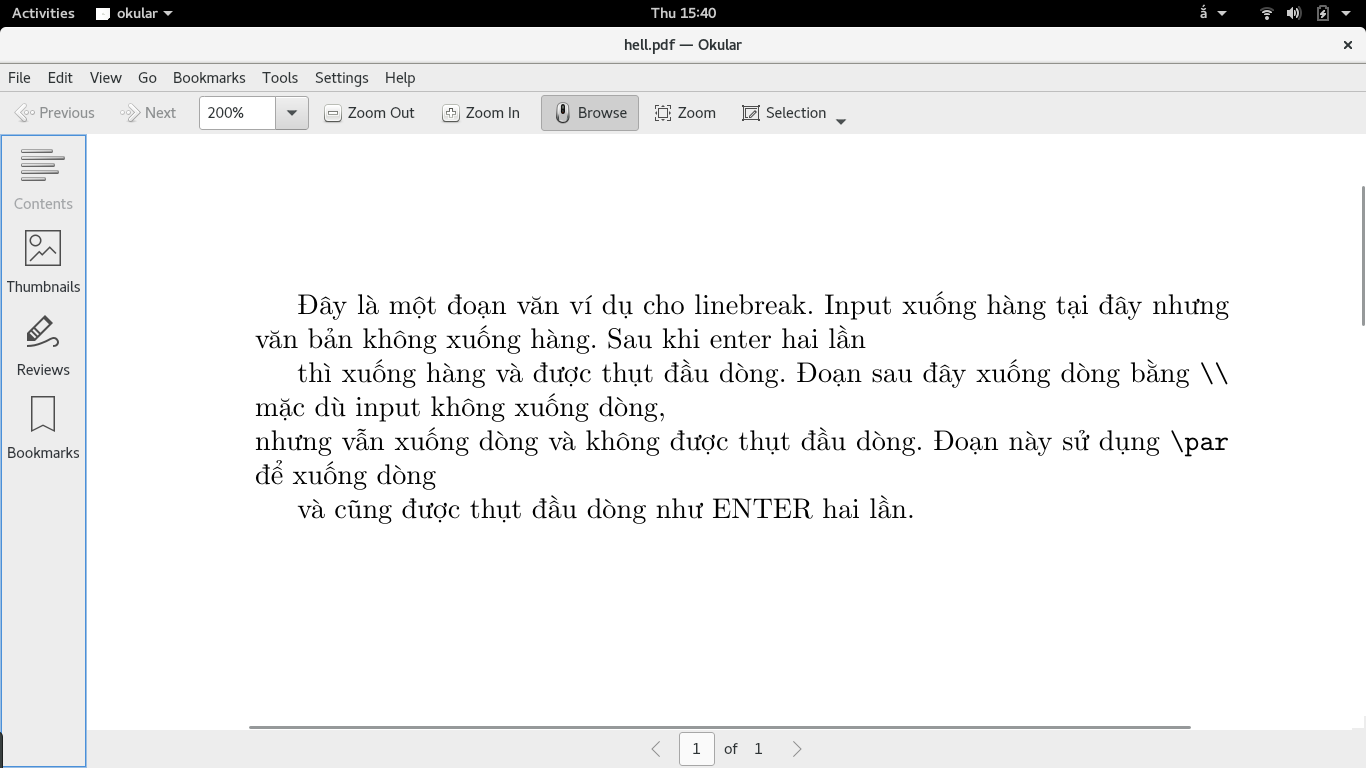
\includegraphics[width=0.9\textwidth]{linebreak}
 \caption{Ví dụ xuống dòng}
 \label{fig:linebreak} 
\end{figure}

Ta thấy văn bản đầu ra chỉ xuống dòng ở những nơi có ENTER hai lần, dấu \verb=\\= và câu lệnh \verb=\par=.
Những nơi có ENTER chỉ một lần, LaTeX không cho xuống dòng và tiếp tục in thẳng cho tới khi hết chiều
dài cho phép của một dòng. ENTER hai lần tương đương với câu lệnh \verb=\par=, ngoài xuống dòng
còn tiến hành canh chỉnh cho đoạn văn tiếp theo, dấu \verb=\\= chỉ đơn thuần là cho xuống dòng.
Ta thấy trong ví dụ hình \ref{fig:linebreak}, sau ENTER hai lần, dòng đầu của đoạn cũng thụt vào như \verb=\par=.\par 
Mặc định, văn bản Latex luôn ở chế độ canh đều (justify), nhưng nếu chúng ta muốn canh trái, phải hoặc
giữa, LaTeX cũng cung cấp các câu lệnh và môi trường cho việc đó như ví dụ sau ở hình \ref{fig:align}:
\clearpage 
\begin{verbatim}
\begin{center}
Hello, here is some text without a meaning. This text should show what 
a printed text will look like at this place. If you read this text, 
you will get no information.  
\end{center}

\begin{flushleft}
Hello, here is some text without a meaning. This text should show what 
a printed text will look like at this place. If you read this text, 
you will get no information.  
\end{flushleft}

\begin{flushright}
Hello, here is some text without a meaning. This text should show what 
a printed text will look like at this place. If you read this text, 
you will get no information. 
\end{flushright}
\end{verbatim}
\begin{figure}[H]
 \centering
 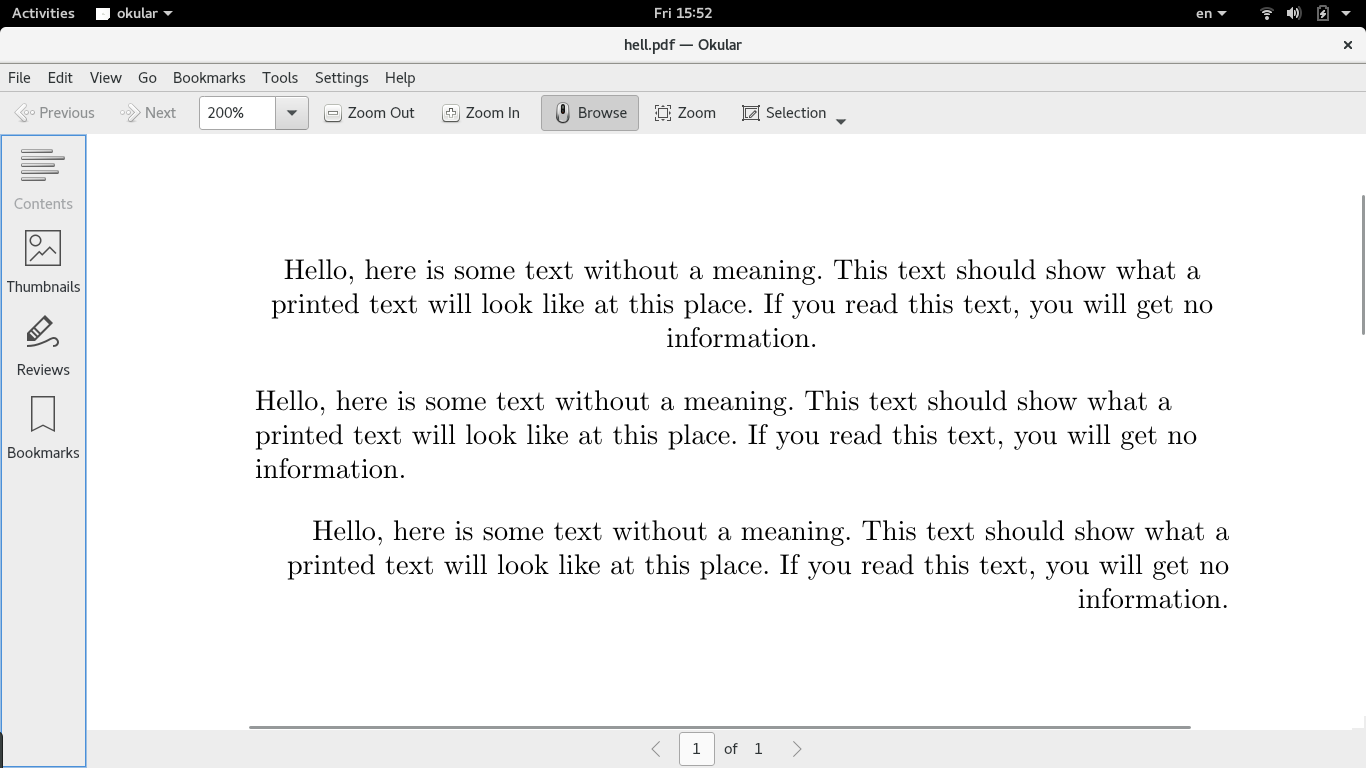
\includegraphics[width=0.9\textwidth]{align}
 \caption{Ví dụ canh vị trí}
 \label{fig:align} 
\end{figure}

Như có thể thấy, ta chỉ cần đặt đoạn văn bản cần cân chỉnh vào giữa hai câu lệnh \path|\begin{env}...\end{env}|,
trong đó \textsl{env} là tên của môi trường (environment) canh chỉnh: \textbf{\slshape center, flushleft} hoặc \textbf{\slshape flushright}.\par
\subsubsection*{Thêm hình ảnh và tạo bảng}
Dưới đây là đoạn input ví dụ cho việc thêm hình ảnh.\par
\begin{verbatim}
\documentclass{article}
\usepackage{graphicx}
\graphicspath{ {image/} }

\begin{document}
\begin{figure}[h]
\centering

\includegraphics[width=0.5\textwidth]{logo}
\caption{Example Picture}
\end{figure}
\end{document}
\end{verbatim}
\begin{figure}[H]
 \centering
 
\includegraphics[width=0.9\textwidth]{image}
 \caption{Ví dụ thêm hình trong văn bản}
 \label{fig:image}
\end{figure}

LaTeX cần phải tải (load) gói \hypertarget{graphicx}{\texttt{graphicx}} để thêm hình ảnh, đây là một trong số các gói
cơ bản nên sẽ kèm theo trong gói phân phối của LaTeX. Để sử dụng gói này, ta chỉ việc khai báo
\verb=\usepackage{graphicx}=, tiếp theo là khai báo đường dẫn chứa tập tin hình bằng câu lệnh
\verb=\graphicspath{...}= trong phần tiền tố. Tại vị trí cần thêm hình, ta sử dụng môi trường 
\textbf{\slshape figure} với cú pháp \path|\begin{figure}[placement]...\end{figure}|, trong đó,
\textsl{placement} là vị trí đặt hình, ví dụ ở hình \ref{fig:image} sử dụng \texttt{\bfseries h}, tức đặt hình tại vị trí đặt câu lệnh
(so với các đối tượng khác trong tập tin \texttt{.tex}). \verb=\includegraphics[option]{name}= chính là câu
lệnh thêm hình ảnh, với \textsl{option} ta có thể tuỳ chỉnh thông số (không bắt buộc) cho hình 
dưới dạng từ khoá-giá trị, ví dụ \verb|width=0.9\textwidth|, tức chiều rộng hình bằng 0.9 chiều dài tối đa của 1
dòng trong văn bản, và \textsl{name} là tên hình ảnh ta muốn thêm. Câu lệnh \verb=\caption{}= cho phép
ta đặt chú thích cho hình, câu lệnh sẽ tự động đánh số và nhãn (label) tuỳ theo ngôn ngữ hiện hành,
ở ví dụ \verb=\caption= tự động điền label “Figure 1” trước chú thích hình.\par
Tiếp tục xét ví dụ tạo bảng trong LaTeX.\par
\begin{verbatim}
\begin{center}
\begin{tabular}{ |c|c|c| } 
 \hline
 cell1 & cell2 & cell3 \\ 
 cell4 & cell5 & cell6 \\ 
 cell7 & cell8 & cell9 \\ 
 \hline
\end{tabular}
\end{center}
\end{verbatim}
\begin{figure}[H]
 \centering
 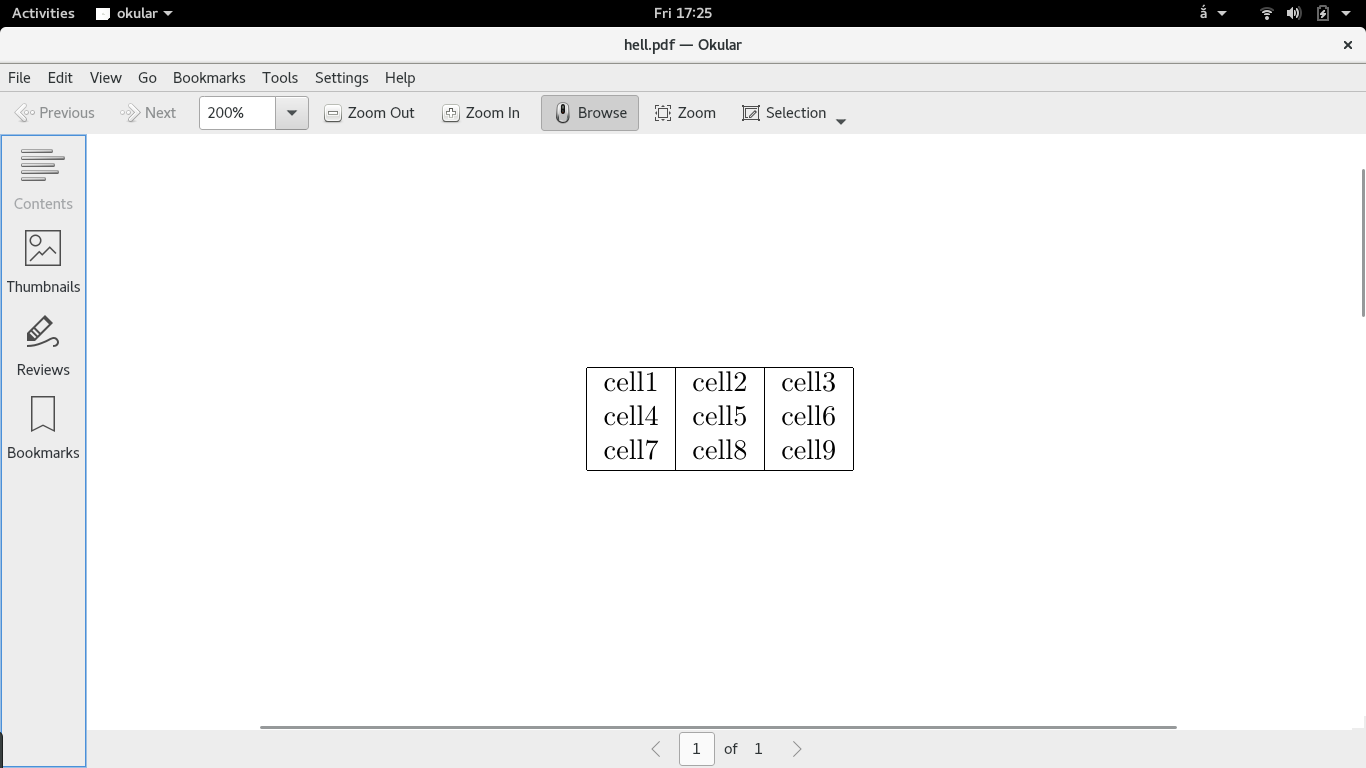
\includegraphics[width=0.9\textwidth]{table}
 \caption{Ví dụ tạo bảng}
 \label{fig:table}
\end{figure}
Ta sử dụng môi trường \hypertarget{table}{\textsl{\bfseries tabular}} để tạo bảng với cú pháp \path=\begin{tabular}{cols}...\end{tabular}=,
trong đó, \textsl{cols} là nơi ta khai báo số cột, canh chỉnh (trái, phải, giữa) và đường phân cách.
Trong ví dụ ở hình \ref{fig:table}, \verb={ |c|c|c| }= ngụ ý bảng có 3 cột, nội dung của cột được canh giữa (center), ngoài \texttt{\bfseries c} ta
còn có các khai báo khác như \texttt{\bfseries l} và \texttt{\bfseries r} ứng với trái (left) và phải (right), kí hiệu | ám chỉ giữa
mỗi cột sẽ có một đường gạch đơn dọc phân cách. Trong môi trường \textsl{\bfseries tabular}, ta tiến hành
soạn nội dung bảng với \& đánh dấu sang cột mới và \verb=\\= đánh dấu sang dòng mới. \verb=\hline=
là câu lệnh báo LaTeX thêm đường kẻ ngang (ở vị trí đặt câu lệnh) cho bảng.\par 
Để biết thêm nhiều câu lệnh liên quan tới việc thêm hình ảnh và tạo bảng, người dùng có thể tham khảo
thêm tại trang web hướng dẫn của \href{https://www.sharelatex.com/learn}{ShareLaTeX} hoặc \cite{lamport} và \cite{latex-comp}.\par
\subsubsection*{Chương và đề mục}
Mỗi loại văn bản sẽ có cấu trúc sắp xếp nội dung khác nhau, tuy nhiên cách sắp xếp cơ bản
nhất vẫn là chương (chapter) và đề mục (section).\par
\begin{verbatim}
\chapter{First Chapter}
 
\section{Introduction}
 
This is the first section.
 
Lorem  ipsum  dolor  sit  amet,  consectetuer  adipiscing  
elit.   Etiam  lobortisfacilisis sem.  Nullam nec mi et 
neque pharetra sollicitudin.  Praesent imperdietmi nec ante. 
Donec ullamcorper, felis non sodales...
 
\section{Second Section}
 
Lorem ipsum dolor sit amet, consectetuer adipiscing elit.  
Etiam lobortis facilisissem.  Nullam nec mi et neque pharetra 
sollicitudin.  Praesent imperdiet mi necante...
 
\subsection{First Subsection}
Praesent imperdietmi nec ante. Donec ullamcorper, felis non sodales...
 
\section*{Unnumbered Section}
Lorem ipsum dolor sit amet, consectetuer adipiscing elit. 
\end{verbatim}
\begin{figure}[H]
 \centering
 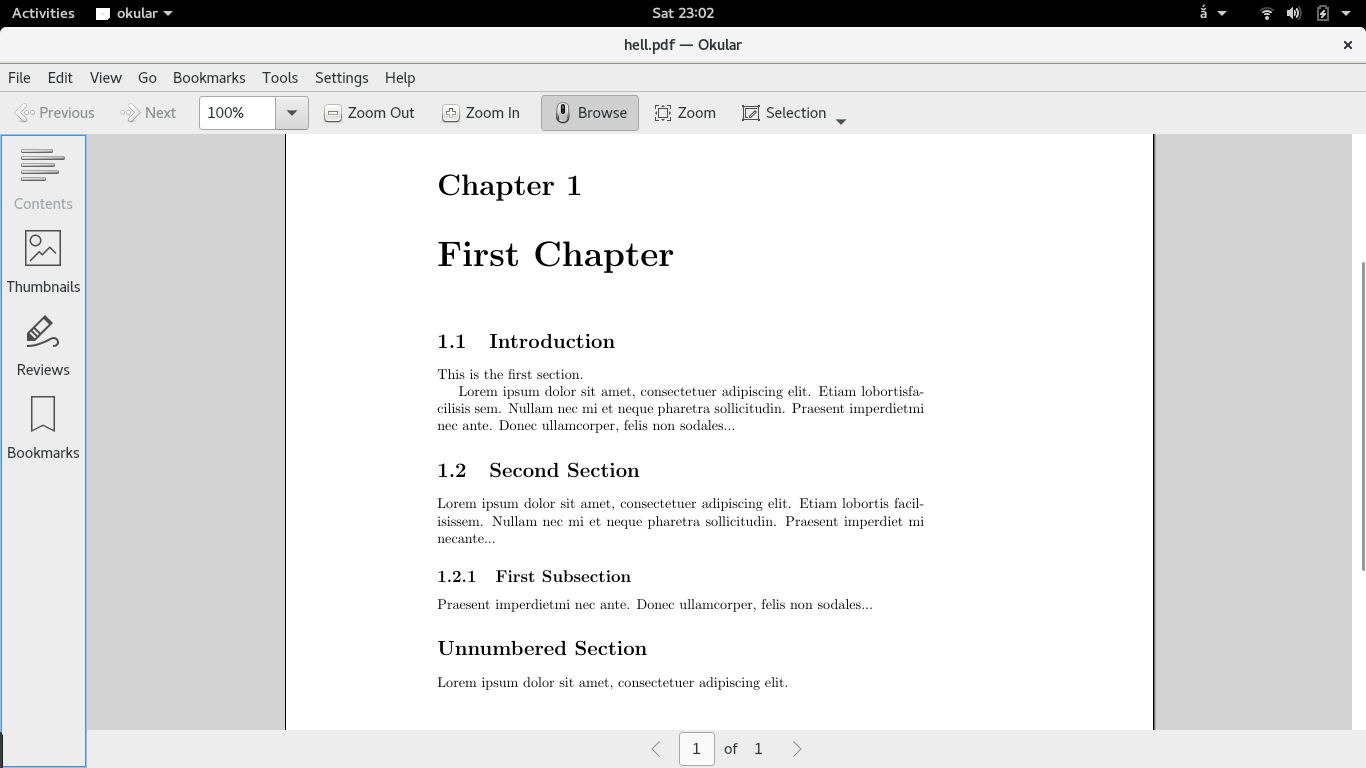
\includegraphics[width=0.9\textwidth]{chapter}
 \caption{Đánh dấu chương và đề mục}
 \label{fig:chapter}
\end{figure}

Câu lệnh \verb=\chapter{title}= và \verb=\section{title}= đánh dấu bắt đầu một chương và mục,
với \textit{title} là tiêu đề của chương, mục đó. LaTeX sẽ tự động tiến hành định dạng cho tiêu
đề và đánh số. Nếu không muốn đánh số ta có thể thêm dấu * vào câu lệnh như ví dụ hình \ref{fig:chapter}
với câu lệnh \verb=\section*=. Ngoài \verb=\chapter= và \verb=\section=, LaTeX còn có
các câu lệnh chia đề mục khác ứng với thứ bậc như sau:\par
\begin{table}[H]
 \centering
 \begin{tabular}{ |l|l| }%
  \hline
  \multicolumn{1}{|c}{Thứ bậc} & \multicolumn{1}{|c|}{Câu lệnh} \\
  \hline
  -1 & \verb=\part{}= \\
  0  & \verb=\chapter{}= \\
  1  & \verb=\section{}= \\
  2  & \verb=\subsection{}= \\
  3  & \verb=\subsubsection{}= \\
  4  & \verb=\paragraph{}= \\
  5  & \verb=\subparagraph{}= \\
  \hline
 \end{tabular}
 \caption{Các câu lệnh chương mục và thứ bậc}
 \label{tab:chapter}
\end{table}

\textbf{Chú ý}: \verb=\part= và \verb=\chapter= chỉ có trong lớp văn bản \verb=report= và \verb=book=.\par

